\documentclass[11pt]{article}
\usepackage{tikz}
\usepackage{pgf-umlcd}
\begin{document}
\section*{Programaci\'{o}n orientada a objetos}
La siguiente f\/igura muestra parte de un diagrama de clases correspondiente a un 
editor de gr\'{a}ficos, que se utilizar\'{a} como ejemplo, a lo largo de esta 
actividad pr\'{a}ctica. El programa a construir debe permitir realizar dibujos 
a partir de cuadros y c\'{i}rculos. Cuando se ejecute el programa se deber\'{a}n 
mostrar Formas en una ventana. La ventana contendr\'{a} un conjunto de Formas. En 
esta versi\'{o}n del programa, los Items son una generalización de una Forma. Las 
Formas pueden ser Cuadros o C\'{i}rculos.
\begin{center}
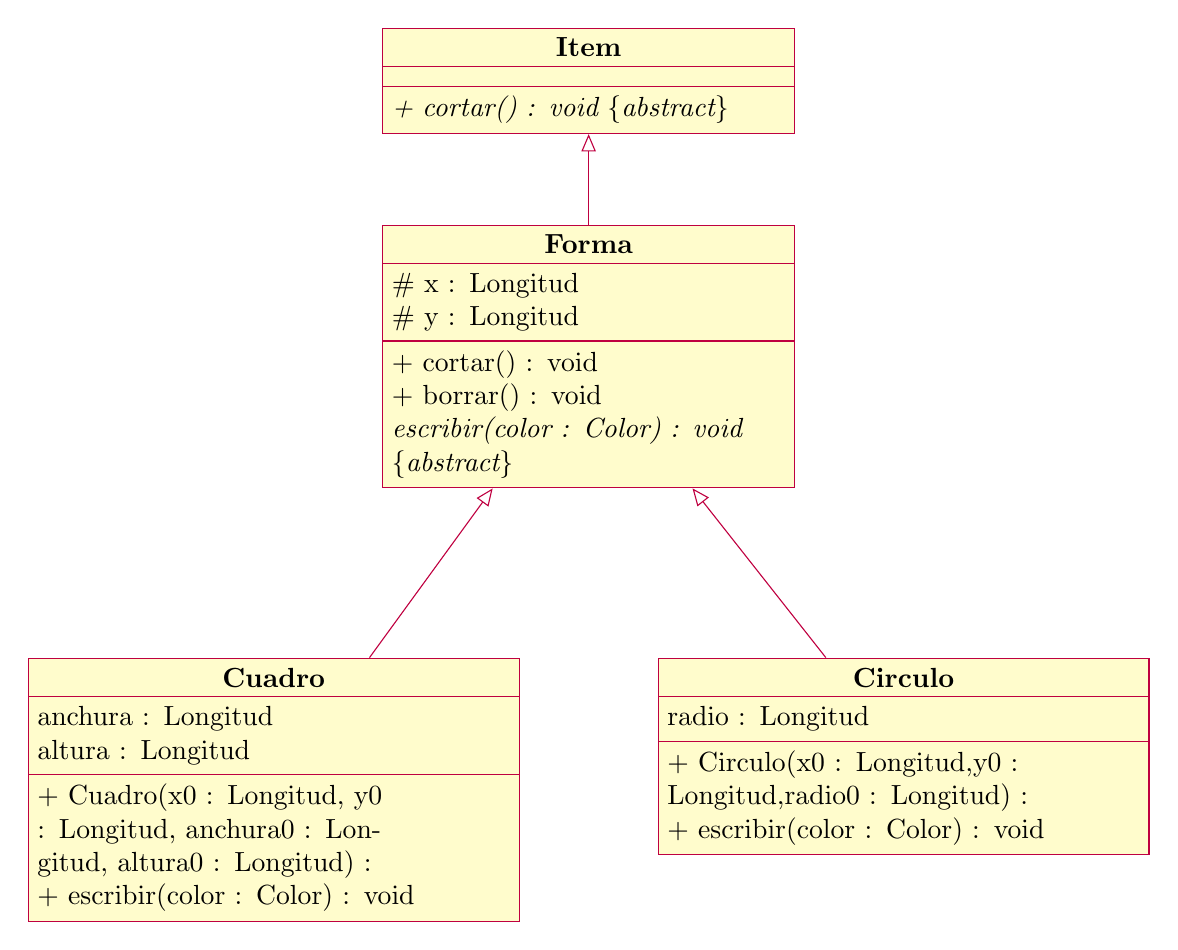
\begin{tikzpicture}
  \begin{class}[text width=5cm]{Item}{0,0}
    \operation[0]{+ cortar() : void $\{$abstract$\}$}
  \end{class}
  \begin{class}[text width=5cm]{Forma}{0,-2.5}
    \inherit{Item}
    \attribute{\# x : Longitud}
    \attribute{\# y : Longitud}
    \operation{+ cortar() : void }
    \operation{+ borrar() : void}
    \operation[0]{escribir(color : Color) : void $\{$abstract$\}$}
  \end{class}
  \begin{class}[text width=6cm]{Cuadro}{-4,-8}
    \inherit{Forma}
    \attribute{anchura : Longitud}
    \attribute{altura : Longitud}
    \operation{+ Cuadro(x0 : Longitud, y0 : Longitud, anchura0 : Longitud, altura0 : Longitud) : }
    \operation{+ escribir(color : Color) : void}
  \end{class}
  \begin{class}[text width=6cm]{Circulo}{4,-8}
  \inherit{Forma}
  \attribute{radio : Longitud}
  \operation{+ Circulo(x0 : Longitud,y0 : Longitud,radio0 : Longitud) : }
  \operation{+ escribir(color : Color) : void}
  \end{class}
\end{tikzpicture}
\end{center}
En pr\'{o}ximas versiones de este documento se mostrar\'{a}n esqueletos de c\'{o}digo, a partir 
de los cuales se podr\'{a} construir la versi\'{o}n del programa aqu\'{i} descrito. 
\end{document}